\section{Tělo trezoru}
Dveře trezoru (o kterých je většina této práce) jsou schopny se zamknout do čehokoli se správným tvarem vstupního otvoru. 
Proto je možné velice jednoduše navrhnout libovolnou skříň, které by dveře sloužily jako zamykatelné víko. 

Aby trezor mohl sloužit (alespoň teoreticky) jako opravdový trezor a~ne jen jako hračka, navrhl jsem i bezpečnostní schránku, která by se zazdila do zdi. 

Vzhledem k~velikosti dveří by totiž ani nedobytná schránka nebyla bezpečná, jelikož by se dala jednoduše přenést celá.

\begin{figure}[htbp]
    \centering
    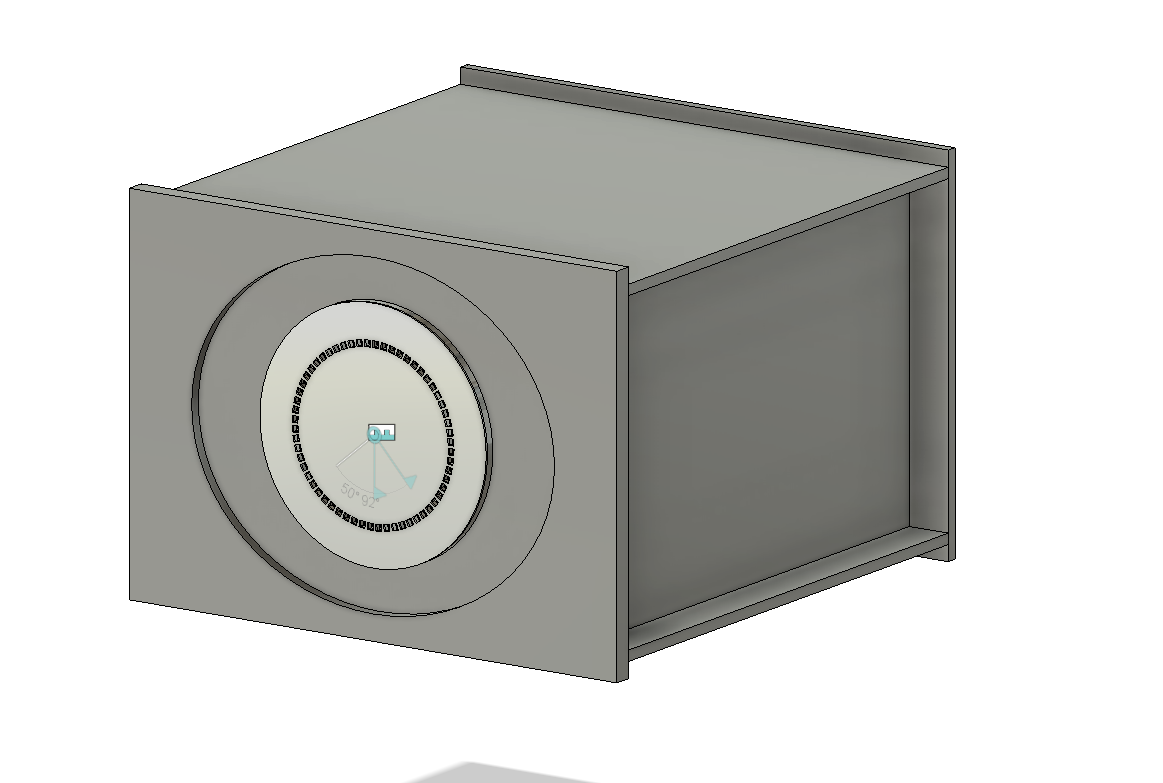
\includegraphics[width=240pt]{kapitoly/obrazky/E4/bedna/bedna.png}
    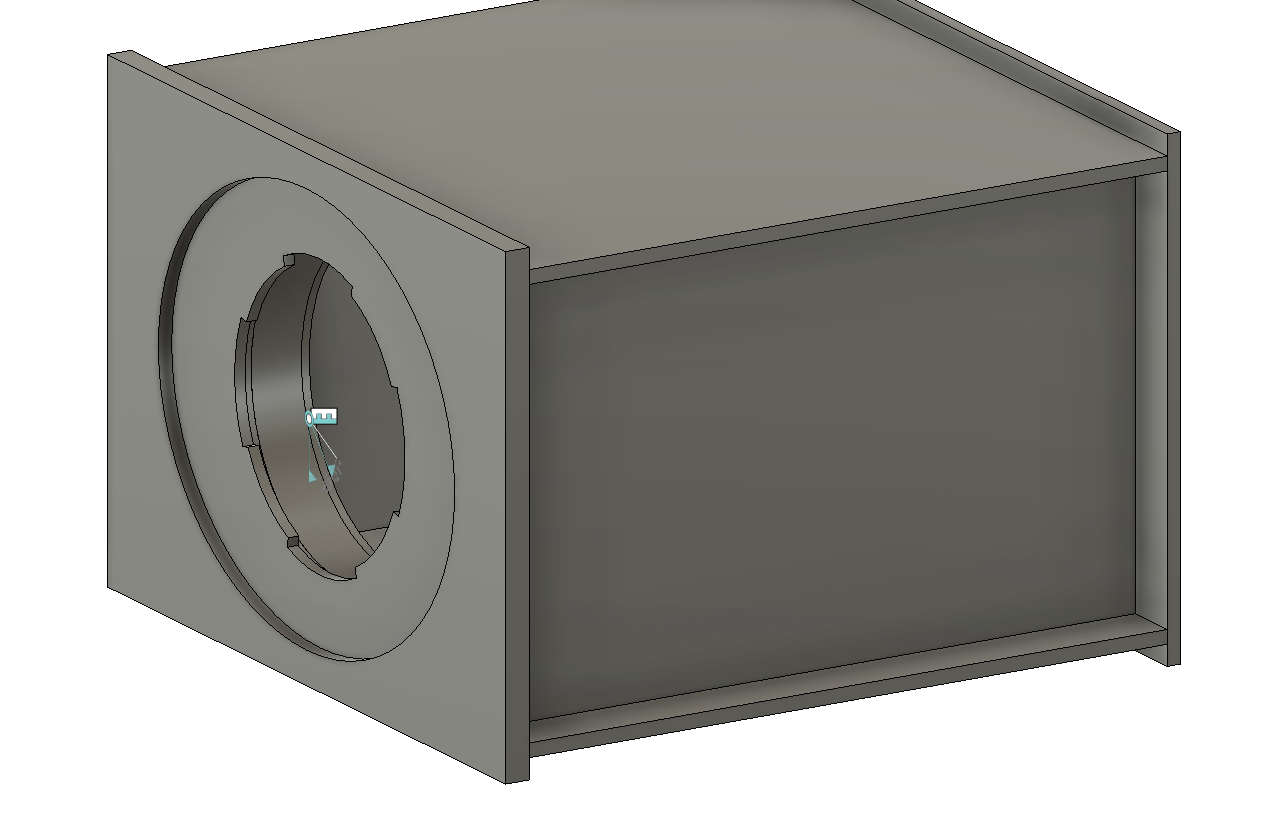
\includegraphics[width=240pt]{kapitoly/obrazky/E4/bedna/jen-bedna.png}
    \caption{Render bezpečnostního těla trezoru}
    \label{fig:E4-bedna}
\end{figure}

Tato bezpečnostní schránka by měla mít odolnou přední stěnu, ostatní stěny by pak měly zajišťovat jen pevné uchycení ve stěně.
Uchycení je tedy zajištěno tvarem schránky. Pro vyjmutí trezoru by tak bylo potřeba vybourat část zdi.
\enlargethispage{5mm}

Pro co možná největší bezpečnost by tedy bylo nutné přední stěnu trezoru alespoň zarovnat (lépe zahloubit) s povrchem stěny.
Zadní stěnu by pak bylo nutné umístit do prostoru zdi tak, aby nebylo snadné se probourat skrz tuto stěnu z druhé strany zdi.